\section{Introduction}
\label{sec:intro}

Being able to automatically describe the content of an image using properly
formed English sentences is a very challenging task, but it could have great
impact, for instance by helping visually impaired people better understand the
content of images on the web. This task is significantly harder, for example, than the
well-studied image classification or object recognition tasks,
which have been a main focus in the computer vision community~\cite{ILSVRCarxiv14}.
Indeed, a description must capture not only the objects contained in an image, but
it also must express how these objects relate to each other as
well as their attributes and the activities they are involved in. Moreover, the above
semantic knowledge has to be expressed in a natural language like English, which
means that a language model is needed in addition to visual understanding.

Most previous attempts have proposed
to stitch together existing solutions of the above sub-problems, in order to go from
an image to its description~\cite{farhadi2010every,kulkarni2011baby}. In contrast, we would like to 
present in this work a single joint model that
takes an image $I$ as input, and is trained to maximize the likelihood
$p(S|I)$ of producing a target sequence of words $S = \{S_1, S_2, \ldots\}$
where each word $S_t$ comes from a given dictionary, that describes the image
adequately.

\begin{figure}
\begin{center}
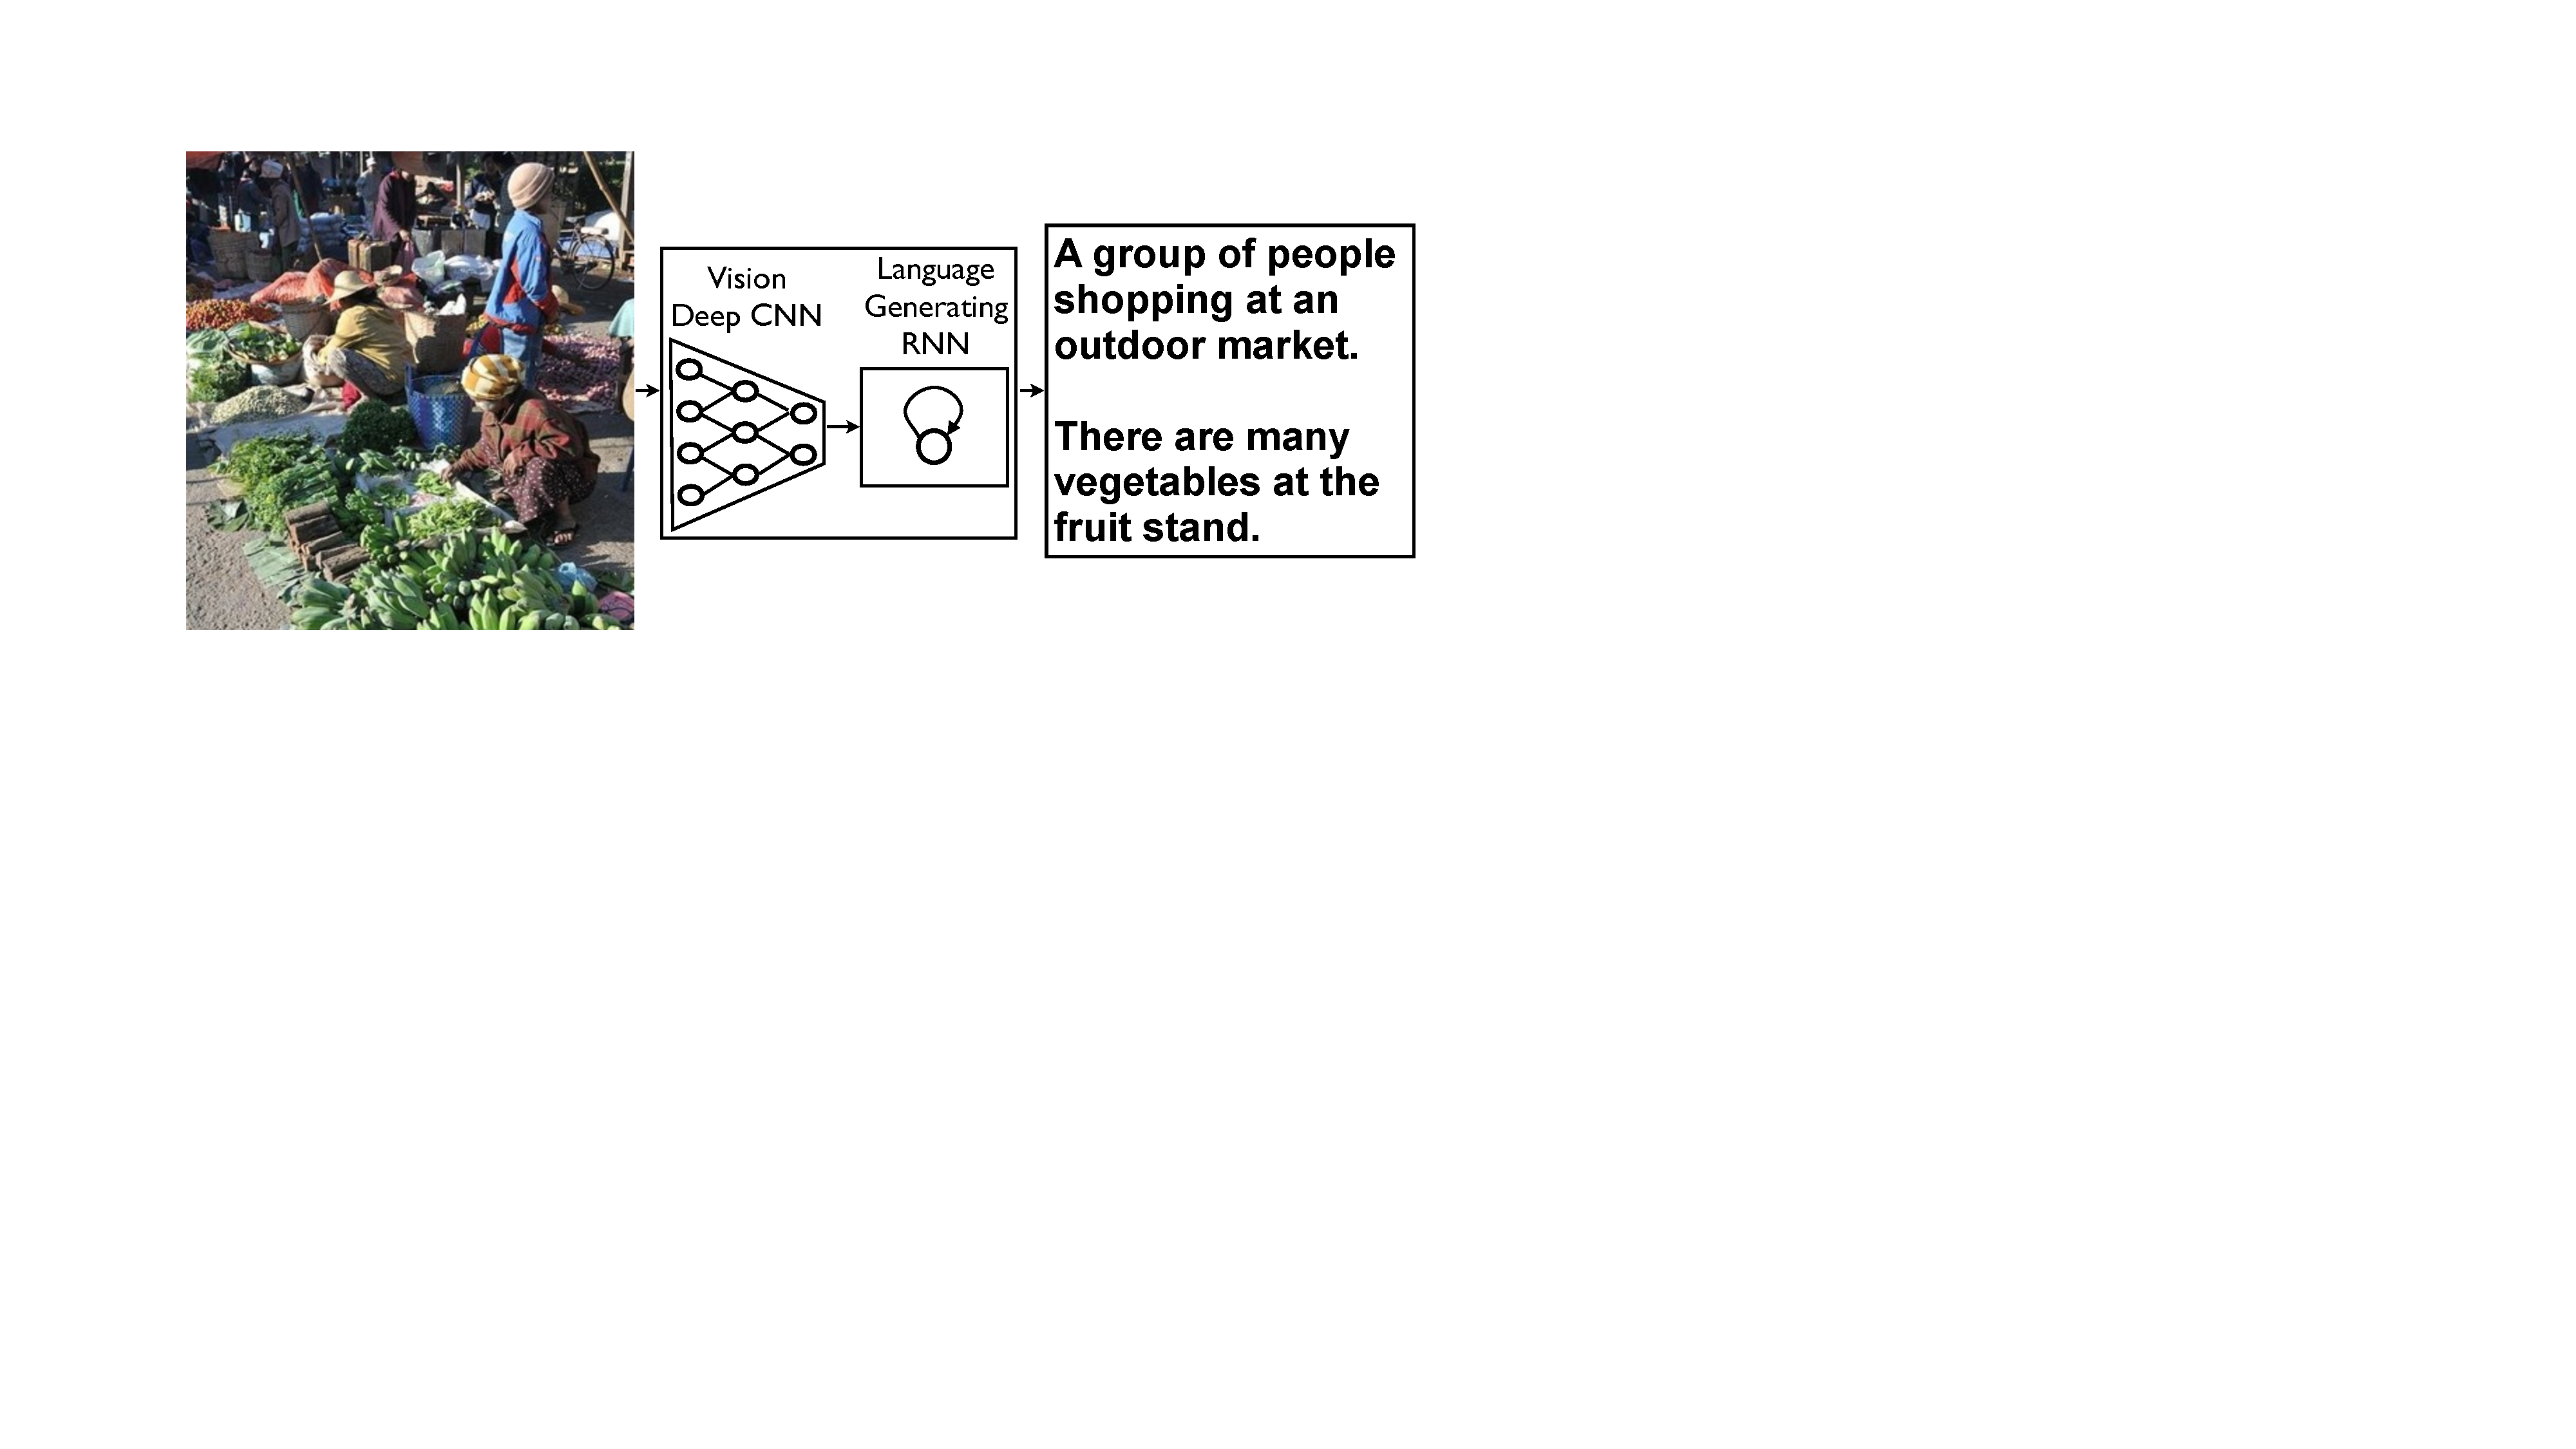
\includegraphics[width=0.5\textwidth]{overview_fig_2.pdf}
\end{center}
\caption{\label{fig:overview} NIC, our model, is based end-to-end on a neural network consisting of a vision CNN followed by a language generating RNN. It generates complete sentences in natural language from an input image, as shown on the example above.}
\end{figure}


The main inspiration of our work comes from recent advances in machine translation, where the task is to transform a sentence $S$ written
in a source language, into its translation $T$ in the target language, by
maximizing $p(T|S)$. For many
years, machine translation was also achieved by a series of separate tasks
(translating words individually, aligning words, reordering, etc), but recent
work has shown that translation can be done in a much simpler way using 
Recurrent Neural Networks
(RNNs)~\cite{cho2014learning,bahdanau2014neural,sutskever2014sequence}
and still reach state-of-the-art performance.
An ``encoder'' RNN {\em reads} the source sentence and
transforms it into a rich fixed-length vector representation, which in turn in used as the 
initial hidden state of a ``decoder'' RNN that {\em generates}
the target sentence.

Here, we propose to follow this elegant recipe,
replacing the encoder RNN by a deep convolution neural network (CNN). Over the last few years it has been convincingly 
shown that CNNs can produce a rich representation of the input image by embedding it
to a fixed-length vector, such that this representation can be used for a variety of
vision tasks~\cite{sermanet2013overfeat}. Hence, it is natural to use a CNN as an
image ``encoder'', by first pre-training it for an image classification task and
using the last hidden layer as an input to the RNN decoder that generates sentences (see Fig.~\ref{fig:overview}).
We call this model the Neural Image Caption, or NIC.

Our contributions are as follows. First, we present an end-to-end system for the
problem. It is a neural net which is fully trainable using stochastic
gradient descent.
Second, our model combines state-of-art sub-networks for vision and language models. These
can be pre-trained on larger corpora and thus can take advantage of additional data. Finally,  
it yields significantly better performance compared to state-of-the-art approaches;
for instance, on the Pascal dataset, NIC yielded a BLEU score of 59,
to be compared to the current state-of-the-art of 25, while human performance
reaches 69. On Flickr30k, we improve from 56 to 66, and on SBU,
from 19 to 28.
